\documentclass[a4paper,12pt]{article} % тип документа

% Поля страниц
\usepackage[left=2.5cm,right=2.5cm, top=2cm,bottom=2cm,bindingoffset=0cm]{geometry}
    
%Пакет дял таблиц   
\usepackage{multirow} 
    
%Отступ после заголовка    
\usepackage{indentfirst}

\usepackage{float}
\usepackage{multirow}


% Рисунки
\usepackage{subcaption,floatrow,graphicx,calc}
\usepackage{wrapfig}

% Создаёем новый разделитель

% Ссылки?
\usepackage{hyperref}
\usepackage[rgb]{xcolor}
\hypersetup{				% Гиперссылки
    colorlinks=true,       	% false: ссылки в рамках
	urlcolor=blue          % на URL
}


%  Русский язык
\usepackage[T2A]{fontenc}			% кодировка
\usepackage[utf8]{inputenc}			% кодировка исходного текста
\usepackage[english,russian]{babel}	% локализация и переносы


% Математика
\usepackage{amsmath,amsfonts,amssymb,amsthm,mathtools, mathrsfs, wasysym}


\begin{document}
\begin{center}
	\footnotesize{ФЕДЕРАЛЬНОЕ ГОСУДАРСТВЕННОЕ АВТОНОМНОЕ ОБРАЗОВАТЕЛЬНОЕ 			УЧРЕЖДЕНИЕ ВЫСШЕГО ОБРАЗОВАНИЯ}\\
	\footnotesize{МОСКОВСКИЙ ФИЗИКО-ТЕХНИЧЕСКИЙ ИНСТИТУТ\\(НАЦИОНАЛЬНЫЙ 			ИССЛЕДОВАТЕЛЬСКИЙ УНИВЕРСИТЕТ)}\\
	\hfill \break
	\hfill\break
	\hfill\break
	\hfill \break
	\hfill \break
	\hfill \break
	\hfill \break
	\hfill \break
	\hfill \break
	\hfill \break
	\hfill \break
	\hfill \break
	\hfill \break
	\hfill \break
	\large{Лабораторная работа № 5.5.1 \\\textbf{Измерение коэффициента ослабления потока $\gamma$-лучей в веществе и опредление их энерегии.}}\\
	\hfill \break
	\hfill \break
	\hfill \break
	\begin{flushright}
		Мельникова Юлия\\
        Калинин Даниил\\
		Группа Б01-108а
	\end{flushright}
	\hfill \break
	\hfill \break
	\hfill \break
	\hfill \break
	\hfill \break
	\hfill \break
	\hfill \break
	\hfill \break
	\hfill \break

\end{center}
\begin{center}
	Долгопрудный, 2023 г.
\end{center}
\thispagestyle{empty}
\newpage


	\subsection*{Аннотация:}
	\begin{enumerate}
		\item С помощью сцинтилляционного счётчика измерить линейные коэффициенты ослабления потока $\gamma$-лучей в свинце, железе, алюминии.
		
		\item По линейным коэффициентам ослабления потока $\gamma$-лучей определить энергию $\gamma$-квантов.
	\end{enumerate}
	
	\subsection*{Описание экспериментальной установки}
	
	Схема экспериментальной установки приведена на рисунке \ref{img:exp_scheme}:
	\begin{figure}[H]
		\centering
		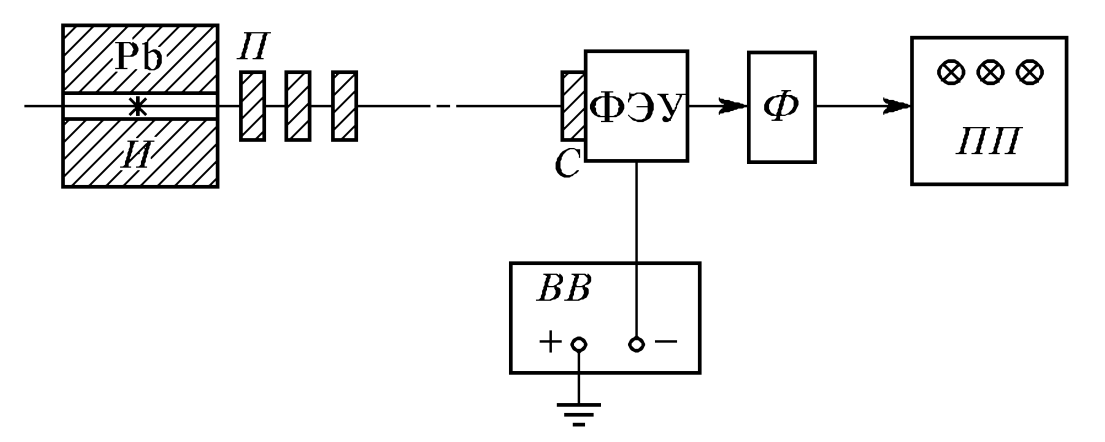
\includegraphics[width=0.5\textwidth]{images/exp_scheme.png}
		\caption{Схема экспериментальной установки.}
		\label{img:exp_scheme}
	\end{figure}

	Источник $\gamma$-лучей И окружён свинцовой оболочкой. Коллиматор выделяет узкий параллельный пучок $\gamma$-квантов, который проходит через набор поглотителей П, и регистрируется сцинтилляционным счётчиком С (кристалл $NaI(Tl)$). Сигнал со счётчика усиливается каскадом фотоэлектронного умножителя и формирователя-выпрямителя Ф, и регистрируется пересчётным прибором ПП. Высоковольтный выпрямитель ВВ обеспечивает питание сцинтилляционного счётчика.
	
	\subsection*{Оборудование}
	
	Экспериментальная установка №5.1б.
	
	\begin{enumerate}
		\item Набор поглотителей из алюминия, свинца и железа. Инвентарный номер №420139237208.
		
		\item Блок детектирования сцинтилляционный РАДЭК БДЕГ-40. Заводской номер №2811. Инвентарный номер №4024.
		
		\item Высоковольтный источник питания Scaler 1403. Инвентарный номер №410134125708.
		
		\item Источник гамма-излучения в свинцовой оболочке.
		
		\item Штангенциркуль. Погрешность измерения равна половине цены деления $\sigma_{\text{шт}} = 0.05$  мм.
	\end{enumerate}

 \newpage
\subsection*{Экспериментальные данные}
 
   \begin{table}[!htb]
    \begin{minipage}{.5\linewidth}
      \centering
        \begin{tabular}{|c|c|c|}
        \hline
        $t$, c &  $n$ & $\sigma_n$ \\ \hline
        120  &  3480  &  59 \\ \hline
        120  &  3444  &  59 \\ \hline
        120  &  3435  &  59 \\ \hline
        120  &  3481  &  59 \\ \hline
        \end{tabular}
    	\centering
    	\caption{Радиационный фон}
    	\label{dark}
    \end{minipage}%
    \begin{minipage}{.5\linewidth}
      \centering
        \begin{tabular}{|c|c|c|}
        \hline
        $t$, c &  $n_0$ & $\sigma_n$ \\ \hline
        60  &  520119  &  721 \\ \hline
        60  &  516950  &  719 \\ \hline
        60  &  516531  &  712 \\ \hline
        60  &  515567  &  718 \\ \hline
        60  &  516086 &  718 \\ \hline
        \end{tabular}
    	\centering
    	\caption{Открытый источник}
    	\label{dark}
    \end{minipage} 
\end{table}

   \begin{table}[!htb]
    \begin{minipage}{.5\linewidth}
      \centering
      \begin{tabular}{|c|c|c|c|c|c|}
    \hline
      $t, c$  & $L,  \text{мм}$ & $\sigma_L, \text{мм}$ & $n$ & $\sigma_n$ \\ \hline
        60  &  20.2  &  0.05  &   338859  &  582 \\ \hline
        60  &  40.4  &  0.05  &   173829  &  417 \\ \hline
        60  &  60.4  &  0.05  &   145886  &  382 \\ \hline
        60  &  80.2  &  0.05  &    97746  &  313 \\ \hline
        60  &  100.4  &  0.05  &    65171  &  255 \\ \hline
    \end{tabular}
	\centering
	\caption{Поглотитель из алюминия}
	\label{dark}
    \end{minipage}%
    \begin{minipage}{.5\linewidth}
      \centering
    \begin{tabular}{|c|c|c|c|c|c|}
    \hline
      $t, c$  & $L,  \text{мм}$ & $\sigma_L, \text{мм}$ & $n$ & $\sigma_n$ \\ \hline
        60  &  10.6  &  0.05  &   292907  &  541 \\ \hline
        60  &  20.8  &  0.05  &   160565  &  400 \\ \hline
        60  &  31.0  &  0.05  &    90941  &  302 \\ \hline
        60  &  41.2  &  0.05  &    50856  &  226 \\ \hline
        60  &  51.6  &  0.05  &    28198  &  168 \\ \hline
    \end{tabular}
	\centering
	\caption{Поглотитель из железа}
	\label{dark}
    \end{minipage} 
\end{table}

\begin{table}[h!]
    \begin{tabular}{|c|c|c|c|c|c|}
    \hline
      $t, c$  & $L,  \text{мм}$ & $\sigma_L, \text{мм}$ & $n$ & $\sigma_n$ \\ \hline
        60  &  4.5  &  0.05  &   295683  &  544 \\ \hline
        60  &  9.2  &  0.05  &   167728  &  410 \\ \hline
        60  &  14.1  & 0.05  &    96834  &  311 \\ \hline
        60  &  19.0  & 0.05  &    54374  &  233 \\ \hline
        60  &  23.9  & 0.05  &    31137  &  176 \\ \hline
    \end{tabular}
	\centering
	\caption{Поглотитель из свинца}
	\label{dark}
\end{table}

\subsection*{Обработка результатов}
	В условиях нашего эксперимента необходимо учитывать фон, поэтому
	\begin{equation*}
		N_0 = n_0 - n_\text{фон}, \ N = n - n_\text{фон}.
	\end{equation*}
 
    Относительная пограшность измерения фона           $ \varepsilon_{\text{фон}} = 1.107 \%\ $, была определена через коэффициент Стьюдента при доверительном интервале 0.95, умноженный на среднеквадратичную ошибку: $ \varepsilon_{\text{фон}} = t_{0.95} * \sqrt{\frac{\sum_{i=1}^{N}\left(x_i - \bar{x}\right)^2}{N\left(N - 1\right)}}$

    Из проведённой серии измерений взято $N_0 = 517050$, $N_{\text{фон}} = 3460$
    
	Для определения коэффициента ослабления $\mu$ в различных веществах небходимо построить графики  зависимостей $\ln N_0/N$ от $l$. Погрешности определялись следующим образом:
    \begin{center}
		$
		\sigma_N = \sqrt{\sigma_{n}^2 + \sigma_{n_{\text{шум}}}^2}
		$\\
        $
		\sigma_{N/t} = \frac{N}{t} \cdot \varepsilon_{N} = \frac{N}{t} \cdot \frac{\sigma_N}{N}
		$\\
		$
		\sigma_{\ln n} = \frac{1}{n} \cdot \sigma_n
		$\\
	\end{center}
		
	
Построим график зависимости количества зарегистрированных в секунду $\gamma$-квантов $n$ от толщины поглощающего слоя $l$ в обычном и логарифмическом масштабе (рис. 2, 3). Кресты погрешности малы и на первом графике не видны.
	
	\begin{figure}[H]
		\centering
        \centering
        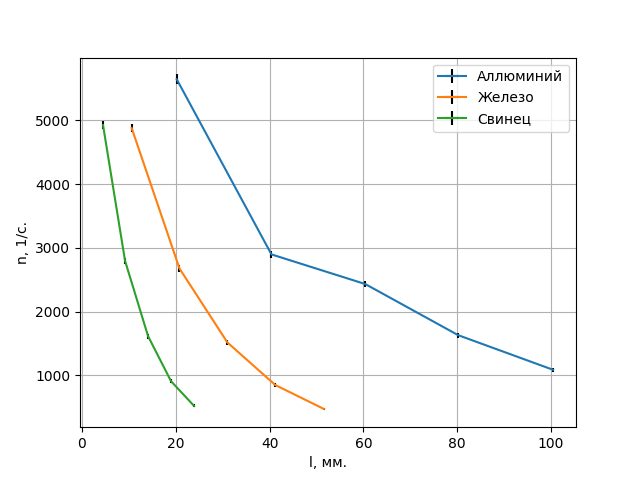
\includegraphics[width=0.7\textwidth]{graph1.png}
        
        \caption{График зависимости $n(l)$.}
        \label{fig:nl}
	\end{figure}
 
 	\begin{figure}[H]
        \centering
        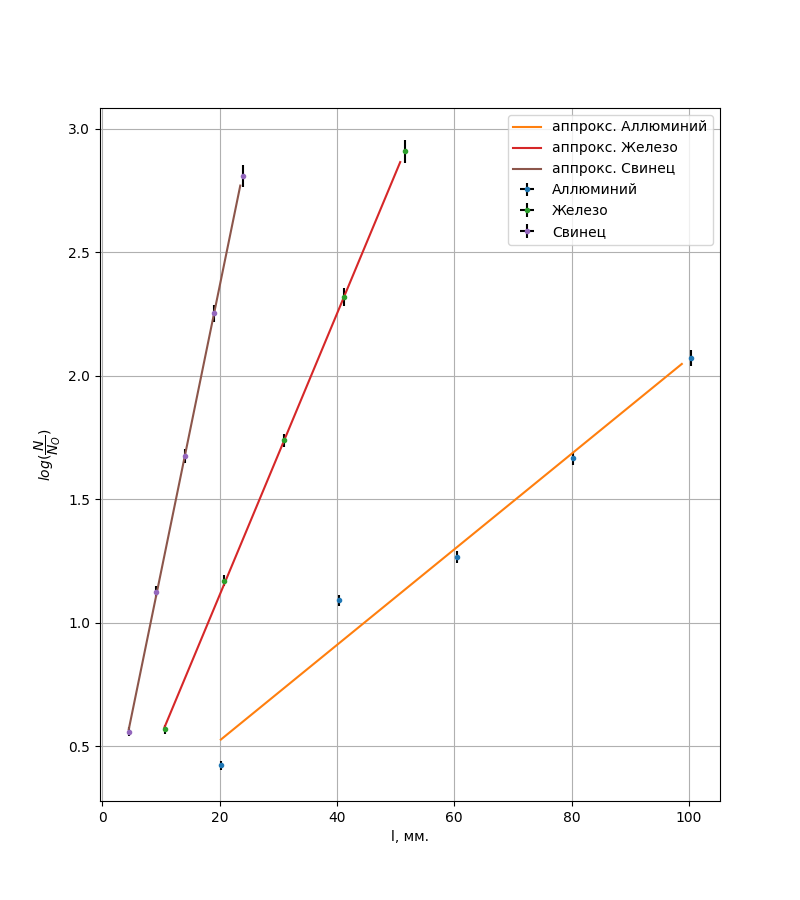
\includegraphics[width=0.7\textwidth]{graph2.png}
        
        \caption{График зависимости $\ln n(l)$.}
        \label{fig:lnnl}
	\end{figure}
		
С помощью метода наименьших квадратов проведём на графике в логарифмическом масштабе прямые. Коэффициенты наклона прямых: \\
	\begin{center}
		$\mu_Pb = 1.16 \pm 0.01 \; {\text{см}}^{-1}$\\
		$\mu_Fe =0.57 \pm 0.01 \; {\text{см}}^{-1}$\\
		$\mu_Al = 0.19 \pm 0.02 \;  {\text{см}}^{-1} $\\
	\end{center}
 
	Определим линейные коэффициенты поглощения, приведённые к плотности вещества:
	$$\mu' = \frac{\mu}{\rho}$$
	
	\begin{center}
		$\mu'_Pb = 0.086 \pm 0.004 \; {\text{см}}^2/ {\text{г}}$\\
		$\mu'_Fe = 0.072 \pm 0.001 \; {\text{см}}^2/ {\text{г}}$\\
		$\mu'_Al = 0.071 \pm 0.001 \;  {\text{см}}^2/ {\text{г}}$\\
	\end{center}

	
	Были взяты следующие значения плотности:\\

	\begin{center}
		$\rho_{Pb} = 13.35 \; {\text{г}} /  {\text{см}}^3 $\\
		$\rho_{Fe} = 7.87  \;  {\text{г}} /  {\text{см}}^3 $\\
		$\rho_{Al} = 2.70 \;   {\text{г}} /  {\text{см}}^3 $\\
	\end{center}
			
\newpage
\subsection*{Обсуждение результатов и выводы}
	В настоящей лабораторной работе с помощью сцинтилляционного счетчика были измерены  линейные коэффициенты ослабления $\mu$ потока $\gamma$-лучей в свинце, железе и алюминии. \\
 
    Табличные значения линейных коэффициентов поглощения:

	\begin{table}[h!]
        \begin{center}
		\begin{tabular}{|c|c|c|c|c|}
			\hline
			$E_\gamma$, МэВ & Pb    & Fe    & Al    \\ \hline
			0,6             & 1,349 & 0,605 & 0,210     \\ \hline
			0,8             & 0,982 & 0,526 & 0,184   \\ \hline
		\end{tabular}
  	\caption{Коэффициенты поглощения $\gamma$-лучей в различных веществах (в~см$^{-1}$).}
		\label{table:spravocka}
         \end{center}
	\end{table}

	Видно, что полученные нами значения коэффициента ослабления потока $\mu$ для каждого вещества лежат в диапазоне энергий от 0,6 МэВ до 0,8 МэВ, поэтому средняя энергия излучения есть $E_\gamma = 0,7$ МэВ.
	
	Заметим, что наклоны прямых на рис. 3 по мере роста заряда ядра увеличиваются. Это связано с природой ослабления $\gamma$-лучей при их прохождении в веществе: фотоэлектрическое поглощение, комптоновское рассеяние, генерация электрон-позитронных пар. Так как $E_\gamma = 0,7 \ \text{МэВ} < 2mc^2$ = 1,02 МэВ, то в нашем случае фотон не может превратиться в электрон-позитронную пару. Комптоновское рассеяние происходит на свободных или слабосвязанных электронах, поэтому, очевидно, сечение не зависит от заряда ядра, откуда $\mu_k \propto Z$. Фотоэффект же в отличии от Комптоновского рассеяния происходит на атоме, и, естественно, что в этом случае сечение уже будет зависеть от заряда ядра. Вообще говоря, строгий квантово-механический рассчет приводит к результату $\sigma_\text{ф} \propto Z^5$. Таким образом, коэффициент ослабления $\gamma$-лучей должен расти при увеличении заряда ядра. 
	

	
\end{document}